\documentclass[twoside,openright,11pt,a4paper]{report}
%\usepackage[T1]{fontenc}
\usepackage[english,francais]{babel}
\usepackage[utf8]{inputenc}
\usepackage[T1]{fontenc}
\usepackage[pdftex]{graphicx}
\usepackage{setspace}
\usepackage{hyperref}
\usepackage[french]{varioref}
%\usepackage[latin1]{inputenc}
%\usepackage{graphicx}
%Options: Sonny, Lenny, Glenn, Conny, Rejne, Bjarne, Bjornstrup
\usepackage[Lenny]{fncychap}
\usepackage{fancyhdr}
\usepackage{fancybox}
\usepackage{a4wide}
\usepackage[chapter]{algorithm}


%\usepackage{algorithm}
%\usepackage{algorithmcx}
\usepackage{algorithmic}
\usepackage{amsmath,amsfonts,amssymb,amsthm}
\usepackage{cases}
%\usepackage[french,english]{babel}
%\usepackage{authblk}
%\usepackage{booktabs}
%\usepackage{bm}
\usepackage{enumerate}
\usepackage{ifthen}
%\usepackage{chapterbib}
%\usepackage{pgfplots,tikz}
%\usepgfplotslibrary{external}
%\usetikzlibrary{external}
%\tikzexternalize[prefix=fig/]
\usepackage{subfig}
\usepackage{pstricks,psfrag}
%\usepackage{notations}
\usepackage{paralist}
\usepackage{xspace}
\usepackage{listings}
%%%%%%%%%%%%%%%%%%%                     ///////////////////
\usepackage{appendix}
%\usepackage{mhchem}
%\usepackage{siunitx}
%\usepackage{multirow}
\usepackage{all}

%\usepackage{refcheck}
%% The following lines should be removed in the final version
%\newboolean{FinalVersion}
%\setboolean{FinalVersion}{false}
%\usepackage{authcomment}

%------------------------------------------------------------------------------%

\graphicspath{{figures/pdf/}}

%------------------------------------------------------------------------------%

\DeclareGraphicsRule{.tif}{png}{.png}{`convert #1 `dirname #1`/`basename #1 .tif`.png}

%------------------------------------------------------------------------------%

\definecolor{dullmagenta}{rgb}{0.4,0,0.4}
\definecolor{darkblue}{rgb}{0,0,0.4}
\definecolor{colKeys}{rgb}{0,0,1}
\definecolor{colIdentifier}{rgb}{0,0,0}
\definecolor{colComments}{rgb}{0,0.5,1}
\definecolor{colString}{rgb}{0.6,0.1,0.1}
%------------------------------------------------------------------------------%

\def\clr{}
\def\clr{_BW}

%------------------------------------------------------------------------------%
 %% Chapter style
%\usepackage{titlesec, blindtext, color}
%\definecolor{gray75}{gray}{0.75}
%\newcommand{\hsp}{\hspace{20pt}}
%\titleformat{\chapter}[hang]{\Huge\bfseries}{\thechapter\hsp\textcolor{gray75}{|}\hsp}{0pt}{\Huge\bfseries}


\usepackage{fancyhdr}

%%%%%%%%%%%%%%%%%%%%%%%%%%%%%%%%%%%%%%%%%%%%%%%%%%%%%%%%

\renewcommand{\chaptermark}[1]{\markboth{Chapitre \thechapter. #1}{}}
\renewcommand{\sectionmark}[1]{\markright{\thesection\ #1}}
\lhead[\fancyplain{}{\bfseries\thepage}]%
      {\fancyplain{}{\bfseries\rightmark}}
\rhead[\fancyplain{}{\bfseries\leftmark}]%
      {\fancyplain{}{\bfseries\thepage}}


%%%%%%%%%%%%%%%%%%%%%%%%%%%%%%%%%%%%%%%%%%%%%%%%%%%%%%%%%%%%%%






\setlength{\headheight}{15pt}

\pagestyle{fancy}
%\renewcommand{\chaptermark}[1]{ \markboth{#1}{} }
%\renewcommand{\sectionmark}[1]{ \markright{#1}{} }

\fancyhf{}
\fancyhead[LE,RO]{\thepage}
\fancyhead[RE]{\textit{ \nouppercase{\leftmark}} }
\fancyhead[LO]{\textit{ \nouppercase{\rightmark}} }

\fancypagestyle{plain}{ %
  \fancyhf{} % remove everything
  \renewcommand{\headrulewidth}{0pt} % remove lines as well
  \renewcommand{\footrulewidth}{0pt}
}
%% http://en.wikibooks.org/wiki/LaTeX/Page_Layout
%%%%%%%%%%%%%%%%%%%%%%%%%%%%%%%%%%%%%%%%%%%%%%%%%%%%%%%%%%%%%%%%%%%%%%%%%%%%%%%%%%%%%%%%%%%%%%%%


\usepackage{ifthen}

\usepackage{minitoc}
\newif \ifPDF
\PDFtrue

%\ifPDF \usepackage[dvips,breaklinks]{hyperref}

\usepackage{graphicx}
%\usepackage[dvips]{graphicx}
%%\usepackage{siunitx}
\usepackage{color}

%\geometry{top=3cm,bottom=3cm,left=2.5cm,right=2.5cm}
                                         
\setcounter{parttocdepth}{2}
\setlength{\ptcindent}{0pt}          
\renewcommand{\ptcfont}{\normalsize\rm} 
\renewcommand{\ptcCfont}{\normalsize\bf}
\renewcommand{\ptcSfont}{\normalsize\rm}


%------------------------------------------------------------------------------%
% Listings

\lstset{
  language        = C++,
  texcl           = true,
  mathescape      = true,
  basicstyle      = \small,
  keywordstyle    = \bf,
  commentstyle    = \it,
  stringstyle     = \color{black!50},
  frame           = {lines}
}

%------------------------------------------------------------------------------%
% Additional macros

\newcommand{\cblue}[1]{{\color{blue}{#1}}}
\newcommand{\cred}[1]{{\color{red}{#1}}}

\DeclareMathOperator{\opcard}{card}
\newcommand{\card}[1]{\opcard(#1)}

%\newcommand{\COO}{CO$_2$\@\xspace}

\newcommand{\setitems}{\mathcal{I}}
\newcommand{\setitem}{I}
\newcommand{\sset}{\mathbb{S}}
\newcommand{\ssetfamily}{\mathcal{S}}


\newcommand{\measd}[2]{|#2|_{#1}}

%% \setcounter{secnumbdepth}{3}
%% \setcounter{tocdepth}{3}
%% \setcounter{minitocdepth}{3}

\DeclareMathOperator{\opdiv}{div}

%------------------------------------------------------------------------------%
% Theorem environments

\newtheorem{example}{Example}
\newtheoremstyle{mystyle}{}{3pt}{\slshape}{}{\scshape}{:\ }{ }{}
\theoremstyle{mystyle}

%------------------------------------------------------------------------------%

%% %----------------------------------------------------------------------------%
%% % mise en page
%% %\pagestyle{Fancy}
%% \pagestyle{fancy}
 
%% \fancyhead{}
%% \fancyfoot{}
 
%% \headheight 62pt
 
%% \fancyhead[LE]{\includegraphics[width=4cm,height=2cm]{figure/index}}
%% \fancyhead[RE]{\includegraphics[width=4cm,height=2cm]{figure/logo_lljl}}

%-------------------------------------------------------------------------


%----------------------------------------------------------------------------%
\numberwithin{equation}{section}

\def\Subm{\rm Submitted}
\def\Submt{\rm Submitted~to~}
\def\Submfp{\rm Submitted for publication}
\def\submfp{\rm submitted for publication}
\def\prep{\rm In~preparation}
\def\toap{\rm to~appear}
\def\Afp{\rm Accepted for publication}
\newif \ifwhere
\def\jour{}



\renewcommand*{\lstlistlistingname}{List of Listings}

%modification interligne
\renewcommand{\baselinestretch}{1.2}
%modification des marges
\addtolength{\hoffset}{0.cm}
\addtolength{\textwidth}{-0.cm}
\addtolength{\voffset}{0cm}
\addtolength{\textheight}{0cm}

%puce itemize text
\renewcommand\FrenchLabelItem{\textbullet}

%\def\thechapter{\Roman{chapter}}
%\usepackage{chapterbib}

\begin{document}

%\dominitoc
\dominitoc
\dominilof
\dominilot


\selectlanguage{french}
\makethese
%\maketitre



%profondeur dans la table des matières et de la numérotation des sections
\setcounter{secnumdepth}{3}
%\setcounter{tocdepth}{3}

%% subsubsection
 
%%

\newpage
\thispagestyle{empty}
\null
\pagenumbering{arabic}
\newpage
%%%%%%%%%%%%%%%%%%%%%%%%%%%%%%%%%%

% {\Large \bfseries Remerciements}
%\phantomsection
%\addcontentsline{toc}{section}{Remerciements}

%\newpage
%\thispagestyle{empty}
%\chapter*{Acknowledgements}
\addtocounter{page}{-1}

\dominitoc
\dominilof
\dominilot
 

 \chapter{Introduction} % Pas de numérotation
%\addcontentsline{toc}{section}{Description} % Ajout dans la table des matières
%\paragraph{Introduction}

Ce pré-rapport décrit mon stage actuellement effectué au sein de l'équipe  APR (Algorithmes, Programmes et Résolution) au laboratoire LIP6 à l'Université Pierre-Et-Marie-Curie sous la direction de M. Emmanuel Chailloux et M. Mathias Bourgoin. Le stage de fin d'étude s'inscrit dans le cadre du Master d'informatique spécialité Systèmes et Applications Répartis (SAR). Il se déroule du 2 février au 31 Juillet 2016.

L'intitulé de mon stage est  \og Exécution parallèle sur cartes graphiques d'un système de gestion de flux de travail de calculs numériques\fg{}, Ce projet est en collaboration avec les universités brésiliennes UFRJ\footnote{UFRJ -   l'Université Fédérale de Rio de Janeiro} et UFF\footnote{UFF - l'Université fédérale Fluminense.}.
\noindent
%\subsection{Organisation du document}
%Ce pré-rapport présente d'abord les systèmes de gestion de workflow scientifique, l'approche algébrique adoptée par ces systèmes, et la programmation GPGPU. Il décrit le contexte de la mission et définit clairement les objectifs de mon stage et sa roadmap générale.

%Une annexe contient les logiciels utilisés dans ce stage.





  \chapter{État de l'art}

Ce chapitre présente le domaine des systèmes de gestion de flux de travail scientifique, l'approche algébrique adoptée par ces systèmes, et les défis rencontrés dans la parallélisation de ces flux. Il introduit également  la programmation GPGPU comme une solution intéressante dans le parallélisme des flux de travail scientifiques. 
%\textbf{Les systèmes de gestion de gestion de flux de travail scientifique}dans un premier temps 

\section{Les systèmes de gestion de flux de travail scientifique}
%Le concept de
%Un gestion de flux de travail scientifique c'est une abstraction pour modéliser et simuler les expériences scientifiques, 

 %manipuler ces gestion de flux de travail (stockage, interrogation, visualisation etc.) %les systèmes des gestion de flux de travail scientifiques sont utilisés pour la gestion des expériences scientifiques où de nombreuses tâches bioinformatiques sont chaînées les unes aux autres,un grand nombre d'outils disponibles pour manipuler ces gestion de flux de travail (stockage, interrogation, visualisation etc.) existe aujourd’hui. 
%ces systèmes représentent les gestion de flux de travail sous la forme d’un graphe pour optimiser le traitement/stockage des informations. 

%On retrouve ainsi 

Le progrès massif dans les différents domaines scientifiques requiert des analyses plus complexes et raffinées sur les expériences scientifiques. Ces expériences à grande échelle sont généralement composées de plusieurs modèles de calcul mathématiques et informatiques. Ils peuvent impliquer l'exécution des simulations sur plusieurs pas de temps, le \textit{fine-tuning} sur un grand ensemble de paramètres. Afin d’assurer une bonne gestion de ces expériences il faut garantir leurs efficacité, cohérence, et reproductibilité \cite{cal}. C’est une tâche très importante mais aussi compliquée compte tenu de la nécessité d'indiquer la provenance des données. Dans le but d'accorder une approche systématique pour modéliser et exécuter de telles expériences, de nombreux domaines scientifiques (comme les services d'informations, et l'analyse de signal) utilisent les systèmes de gestion de flux de travail scientifique (SWfMS) \cite{cal}. Les SWfMS sont des outils pour modéliser et orchestrer l'exécution des flux de travail scientifique. Ils permettent aux utilisateurs de spécifier un flux de travail composé par des activités (programmes informatiques) et par le flux de données entre ces activitées. Cela permet d'enchaîner et de contrôler des différentes tâches pour réaliser un traitement complexe \cite{oga11}. 

% l'exécution en executant des requetes sur la base de données 
%Dans les infrastructures actuelles distribuées, avec des ressources hétérogènes, les systèmes des gestion de flux de travail scientifiques deviennent de plus en plus primordiaux  \cite{cal}. Ils offrent un traitement parallèle et distribué en utilisant soit des ressources informatiques locales, soit un environnement réparti tels que les \textit{clusters}, les grilles ou les \textit{clouds}. 

Dans le cadre de ce stage on s'appuie sur Chiron comme un système de gestion de flux de travail. Chiron (voir Annexe \ref{chiron}) a été crée à l'institue COPPE\footnote{COPPE – Instituto Alberto Luiz Coimbra de Pós-Graduação e Pesquisa de Engenharia.} de l'Université Fédérale de Rio de Janeiro (UFRJ)  avec l'équipe de recherche de Marta Matosso au laboratoire NACAD.
\vspace{0.5cm}
\section[La provenance des données]{La provenance des données dans les systèmes de gestion du flux de travail scientifique  }
L'un des principaux avantages des systèmes de gestion du flux de travail provient de l'enregistrement de la provenance des données. On définit la provenance des données comme des informations qui permettent de déterminer l'historique de dérivation d'un produit de données, à partir de ça source d'origine \cite{sim}. Les deux caractéristiques importantes de la provenance d'un produit de données sont d'une part le produit ancêtre de données à partir de lequel ce produit de données a évolué, et d'autre part le processus de transformation de ce produit ancêtre de données, éventuellement par le biais du flux de travail, qui a aidé à obtenir ce produit de données. Les informations de provenance peuvent être collectées par un modèle orienté processus, où les processus sont les principales entités pour lesquelles la provenance est recueillie, et la provenance des données est déterminée par l'inspection d'entrée et de sortie des produits de données de ces processus.
Si les informations de provenance sont disponibles, ils donnent la possibilité aux utilisateurs d'analyser les résultats de flux de travail, et de décider la dépendance et l'ordonnancement entre les activités de ce flux.
Des requêtes soumises sur les données de provenance peuvent alimenter automatiquement les ensembles de données d'entrée pour un flux de travail en temps d'exécution. L'historique de dérivation des ensembles de données décrit comment le flux de travail a été spécifié et exécuté. Il peut être utilisé pour répliquer les données sur un autre site, ou le mettre à jour si un ensemble de données est périmé en raison de modifications apportées à ses ancêtres.
\vspace{0.5cm}
\section[L'approche algébrique]{L'approche algébrique pour l'exécution parallèle de flux de travail }

%SWfMS tels que Chiron \pageref{chiron} adopte la sémantique des opérateurs algébriques.
 Considérant un flux des tâches avec une dépendance de données entre ces tâches, le modèle d'exécution d'un flux de travail est étroitement couplé à ces spécification \cite{san}. Ce couplage réduit la possibilité d'améliorer les stratégies d'exécution par le système de gestion et par conséquence les améliorations doivent être codées manuellement. Pour répondre à la question de l'optmisation de l'exécution parallèle d'un flux de travail une approche a été proposée dans \cite{oga11}. Elle consiste à abstraire la gestion d'un flux de travail scientifique sous une approche algébrique, inspirée par l'algèbre relationnelle pour les bases de données. Cela fournit un modèle uniform de données qui exprime toutes les données d'une expérience par des relations, chaque combinaison de valeurs des paramètres compose un n-uplet, et les activités de gestion de flux de travail consomment et produisent des n-uplets. Cette abstraction a amélioré la conception et la réutilisation du flux de travail, lorsque les activités sont représentées comme des opérateurs algébriques. Les moteurs de gestion de flux de travail peuvent en outre jouer avec des expressions algébriques équivalentes. Ainsi, les SWfMS identifient la façon dont les données sont structurées et ce qu'il faut attendre de chaque activité, en termes de production et de consommation des données. De cette façon, il est possible d'effectuer des optimisations algébriques et d'adopter des stratégies de distribution intelligentes. 
 

%\paragraph{Chiron}
%(voir Annexe \ref{chiron}) 
%Chiron est un système de gestion de flux de travail de calculs numériques (\textit{scientifique workflow management system}),  il exécute ces simulations comme une chaîne d'activités (programmes) et un flux de données (\textit{dataflow}) sur ces activités. Ce système fournit la gestion des simulations scientifiques, leur exécution parallèle tout en enregistrant la provenance des données. Chiron implémente l'approche algébrique dans un style MapReduce. L'utilisation de MapReduce comme approche de programmation permet aux scientifiques de programmer d'un façon plus simple la procédure du calcul en cachant le parallélisme, qui peut être complexe à gérer \cite{oga13}.

%ratio  Ainsi, l'algèbre soutient naturellement la nature exploratoire des simulations informatiques.
% Les opérateurs excluent les activités de flux de travail en établissant une consommation de données et les critères de production pour chaque activité.
\vspace{0.5cm}
\section[Le parallélisme]{Le parallélisme dans les systèmes de gestion du flux de travail scientifique}
L'ampleur des données produites dans les nombreux domaines scientifiques augmente à un rythme exponentiel, et le progrès de capacité de stockage, de bande passante du réseau, et de puissance de traitement est souvent dépassé. Outre les progrès algorithmiques, la manière canonique pour faire face à l'augmentation des volumes de données est le parallélisme. Cela se reflète dans le développement de l'exécution parallèle des threads sur des puces simples. Ainsi que le développement des infrastructures qui combinent plusieurs machines à des clusters, des grids et des clouds.
%Alors que plusieurs SWfMS comme Dagman et Pegasus (voir Annexe )ont été conçus avec le calcul parallèle sur les ressources partagées, ils fournissent rarement la prise en charge des multicoeur et sont généralement difficile à mettre en place et à utiliser par les scientifiques du domaine. systèmes plus récents comme Taverna mettent davantage l'accent sur la convivialité, mais ne fournissent que des moyens limités vers parallélisation et l'utilisation des ressources informatiques distribuées.
Les réalisations des exécution des flux de travail parallèle sont généralement désignés afin de fonctionner dans ces environnement de calcul particulier.% Généralement, on peut différencier entre trois paramètres: cluster, grids, et clouds.

Une grille informatique (en anglais, grid) est une infrastructure virtuelle constituée d'un ensemble de ressources informatiques potentiellement partagées, distribuées, hétérogènes, délocalisées et autonomes. %Un grid de calcul est un nouveau paradigme de l'informatique distribué dans lequel les ressources de calcul pourraient être hétérogènes et géographiquement éloignés.
Cette infrastructure est qualifiée de virtuelle car les relations entre les entités qui la composent n'existent pas sur le plan matériel mais d'un point de vue logique. L'idée d'un grid est de relier les ressources informatiques afin de résoudre des problèmes de calcul exigeants sans avoir besoin d'un super-ordinateur. Plusieurs SWfMS, tels que Pegasus \cite{pegasus} ou Condor Dagman \cite{condor}, ont été développés pour utiliser les grids pour l'exécution parallèle des flux de travail de calcul intensif.
L’informatique en nuage (en anglais, cloud computing) %décrit une forme de création plus récente de l'informatique distribuée, 
est l'exploitation de la puissance de calcul ou de stockage de serveurs informatiques distants par l'intermédiaire d'un réseau. Ces ressources de calcul et de stockage sont louables sur demande et sur Internet. Le rendement réel des machines virtuelles louées varie considérablement en fonction de la configuration du matériel et de l'utilisation des ressources sous-jacentes partagées  par d'autres utilisateurs. Dans les environnements de grids et de clouds, le transfert important sur des zones étendues des données et les retards dans l'instanciation de grandes quantités des tâches, conduit à une dégradation de performance. 
Un cluster de calcul est un ensemble d'ordinateurs étroitement connectés et fonctionnants comme un système unique. Un nombre toujours croissant de cœurs par processeur et processeurs par cluster ont conduit à un fort potentiel de parallélisation. Puisque les ressources de calcul en clusters sont étroitement couplés, la localité de données est moins problématique par rapport à des environnements distribués, tels que les grids et les clouds. Les clusters fournissent un environnement plus homogène en termes de performances du processeur et de la latence / bande passante entre les n{\oe}uds de calcul. Cependant, l'évolutivité des clusters est limitée et les coûts initiaux d'investissement sont assez élevés, ce qui est problématique.
 %Considérant un flux des tâches avec une dépendance de données entre ces tâches, le modèle d'exécution d'un flux de travail est étroitement couplé à ces spécification \cite{san}. Ce couplage réduit la possibilité d'améliorer les stratégies d'exécution par le système de gestion et par conséquence les améliorations doivent être codées manuellement. 
De toute évidence, l'exécution des flux de travail scientifique présente des défis différents en fonction de l'infrastructure informatique sous-jacente \cite{bux}. 
Les spécifications pour l'exécution en parallèle d'un flux de travail scientifique sont généralement définies avec un langage de script. Ce langage est traitée par un moteur de flux de travail qui génère un plan correspondant pour l'exécution parallèle. Ce plan est une mise en correspondance entre l'architecture parallèle des matériels et la planification des tâches correspondants. Développeurs de flux de travail doivent décider l'ordre, les dépendances et les stratégies de parallélisation. Ces décisions resserrent les possibilités de parallélisation, et peuvent donner à manquer de grandes opportunités d'optimisation.
 Le but de ce stage est d'expérimenter l'accélération GPU comme une nouvelle approche de parallélisme dans le domaine de gestion de flux de travail scientifique. Actuellement, le seul SWfMS qui est en mesure de tirer parti des accélérateurs tels que GPGPU est Swift \cite{kri}. Néanmoins, %, pour tirer profit des GPGPU lors de l'exécution en parallèle, de nouveaux scripts sont nécessaires ou une mapping manuel doit être fait.
La définition de flux de travail dans Swift est fortement couplée à la procédure d'exécution du flux de travail. Et la provenance de données dans Swift est basée sur l'extraction des données à partir des fichiers de logs, de ce fait, le scientifique peut explorer la base de données de provenance uniquement lorsque l'exécution est terminée.
% les coûts initiaux d'acquisition sont assez élevés, ce qui est problématique.
			
		
	

\vspace{0.5cm}
\section{La programmation GPGPU}
 
Les cartes graphiques (GPU) sont des dispositifs performants et spécialisés dotés de nombreuses unités de calcul, dédiés à l'affichage et au traitement 3D. La technologie GPGPU est l'abréviation de \textit{general-purpose computing on graphics processing units}, c'est-à-dire un calcul générique sur un processeur graphique. Cette technologie exploite la puissance de calcul des GPUs pour le traitement massivement parallèle, elle permet d'accélérer les portions de code les plus lourdes en ressources de calcul, en les parallélisant sur de nombreuses unités de calcul, le reste de l'application restant affecté au CPU. La programmation GPGPU offre une accélération très élevée pour un large éventail d'applications scientifiques et commerciales, nettement supérieure à celle offertes par une architecture basée uniquement sur des CPUs \cite{nv}.
Les GPUs offrent une possibilité d'améliorer les exécutions parallèles de flux de travail scientifiques, souvent exprimé avec un grand nombre des tâches de calcul.  % ce qui est très fréquent dans la bio-informatique.
% Explorer dynamiquement les GPUs dans Les tâches concurrentes est une question ouverte, %en particulier dans les flux de travail scientifique exécution parallèle.
Il existe deux outils dédiés à réaliser des calculs généralistes Cuda et OpenCL. Ce sont des outils de très bas niveau d'abstraction, ils demandent de manipuler explicitement de nombreux paramètres matériels. Pour rendre cette t\^ache plus souple et s\^ure, SPOC (voir Annexe \ref{chiron}) est un choix imposé dans le projet. Il consiste à une abstraction haut niveau de la programmation GPGPU. En simplifiant la programmation GPGPU et en autorisant le développement d'optimisations supplémentaires. SPOC nous permet d'atteindre un haut niveau de performance. Il assure aussi la portabilité. Et fournit des squelettes qui peuvent être utilisées pour composer les Kernels \footnote{ Dans la programmation GPU, une fonction définie par l'utilisateur qui tourne sur le GPU est appelé un Kernel.}. Les squelettes sont des constructions algorithmiques basées sur des patrons de conception communs, qui peuvent être paramétrées pour adapter leur comportement. Les squelettes décrivent explicitement les relations entre les kernels et les données. En utilisant cette information, il est possible d'optimiser automatiquement le calcul global \cite{bour14}. Spoc est un outil issue du travail de l'équipe APR du laboratoire LIP6 à l'Université Pierre et Marie Curie. 





%La programmation GPGPU permet d'accélérer les portions de code les plus lourdes en ressources de calcul, en parallélisant les tâches de calcul, le reste de l'application restant affecté au CPU.
 %Les applications s'exécutent ainsi bien plus rapidement \cite{nv}.
%être économes en énergie tout en garantissant une haute performance de calcul grâce à leur capacité de  
 %de calcul de gestion de flux de travail scientifique.
%Technique de programmation visant à l'implantation des applications en exécution sur les cartes graphiques (GPU) au lieu des processeurs centraux (CPU). 
%Technique développée depuis le début des années 2000, où c'est rendu possible l'implantation de programmes sur les adaptateurs graphiques (NVidia, ATI, 3D Labs, ...),

% Enfin, SPOC abstrait les transferts mémoires via l’utilisation de jeux de données spécifiques \cite{tte13}.
%Notre objectif est de construire un environnement d’expérimentation de gestion de flux de travail intégré dans une plateforme 

%Les chercheurs font appel à des supercalculateurs toujours plus rapides en vue d'accélérer le rythme des découvertes et des innovations dans un large éventail de domaines scientifiques

%tourner des applications phénoménalement complexes en temps réel et valide l'utilisation de l'informatique accélérée pour répondre à nos problèmes scientifiques les plus urgents
 
%L'informatique accélérée est l'approche la plus adaptée et la plus réaliste pour parvenir à des niveaux de performance exaflopique dans la décennie à venir." 


%Cette nouvelle fonctionnalité permet aux ingénieurs et aux scientifiques d’accroître les performances de leurs calculs  


%Abstract : Bioinformatics experiments are usually performed using scientific gestion de flux de travail in which tasks are chained together forming very intricate and nested graph structures. Scientific gestion de flux de travail systems have then been developed to guide users in the design and execution of gestion de flux de travail. An advantage of these systems over traditional approaches is their ability to automatically record the provenance (or lineage) of intermediate and final data products generated during gestion de flux de travail execution. The provenance of a data product contains information about how the product was derived, and it is crucial for enabling scientists to easily understand, reproduce, and verify scientific results. For several reasons, the complexity of gestion de flux de travail and gestion de flux de travail execution structures is increasing over time, which has a clear impact on scientific gestion de flux de travail reuse.The global aim of this thesis is to enhance gestion de flux de travail reuse by providing strategies to reduce the complexity of gestion de flux de travail structures while preserving provenance. Two strategies are introduced.First, we propose an approach to rewrite the graph structure of any scientific gestion de flux de travail (classically represented as a directed acyclic graph (DAG)) into a simpler structure, namely, a series-parallel (SP) structure while preserving provenance. SP-graphs are simple and layered, making the main phases of gestion de flux de travail easier to distinguish. Additionally, from a more formal point of view, polynomial-time algorithms for performing complex graph-based operations (e.g., comparing gestion de flux de travail, which is directly related to the problem of subgraph homomorphism) can be designed when gestion de flux de travail have SP-structures while such operations are related to an NP-hard problem for DAG structures without any restriction on their structures. The SPFlow rewriting and provenance-preserving algorithm and its associated tool are thus introduced.Second, we provide a methodology together with a technique able to reduce the redundancy present in gestion de flux de travail (by removing unnecessary occurrences of tasks). More precisely, we detect "anti-patterns", a term broadly used in program design to indicate the use of idiomatic forms that lead to over-complicated design, and which should therefore be avoided. We thus provide the DistillFlow algorithm able to transform a gestion de flux de travail into a distilled semantically-equivalent gestion de flux de travail, which is free or partly free of anti-patterns and has a more concise and simpler structure.The two main approaches of this thesis (namely, SPFlow and DistillFlow) are based on a provenance model that we have introduced to represent the provenance structure of the gestion de flux de travail executions. The notion of provenance-equivalence which determines whether two gestion de flux de travail have the same meaning is also at the center of our work. Our solutions have been systematically tested on large collections of real gestion de flux de travail, especially from the Taverna system. Our approaches are available for use at https://www.lri.fr/~chenj/. 

  
\chapter{Contexte et objectifs}
Ce chapitre décrit le contexte du stage, ces objectifs, ainsi que son plan général.
\section{Contexte}
\label{p2}
Les simulations à grande échelle que l’on rencontre en calculs numériques sont difficiles à gérer. Cela provient de leur nature exploratoire qui nécessite d’évaluer un grand nombre de combinaisons de paramètres, le tout en lançant de nombreuses tâches en parallèle. Les SWfMS ont démontré leurs capacités dans différents domaines scientifiques comme l'astronomie et le biologie \cite{oli}, \cite{dia}, orchestrant la parallélisation des activités de flux de travail \cite{bux}. La programmation GPGPU présente une solution très intéressante dans la parallélisation des milliers d'activités indépendantes, comme dans les opérations de MapReduce. Cependant, il y a plusieurs défis ouverts dans l'exploration des différents modèles de parallélisme pendant l'exécution du flux de travail. Parmi les défis à relever, on s'intéresse ici au problème de l'optimisation de la planification d'exécutions parallèles, laquelle doit tirer profit des architectures hétérogènes (multi-c{\oe}urs, accélérateurs). Par exemple la programmation des cartes graphiques demande un couplage fort entre les unités de calculs parallèles du GPU avec le CPU pour obtenir de bonnes performances, en particulier sur le transfert de données. Les systèmes hétérogènes nécessitent des conceptions complexes combinant différents paradigmes de programmation pour gérer chaque matériel de manière spécifique. 

%Solution SPOC
On cherche alors à abaisser cette complexité dans les flux de travail pour calculs numériques parallèles en utilisant des abstractions de flux de données et des constructions de haut niveau de programmation parallèle pour représenter la spécification du flux de travail et permettre d'optimiser le plan d'exécution parallèle.
 % tout en profitant des différentes architectures multi-core.

%However, there are several open challenges in exploring different models of parallelism during the workflow execution. Among the challenges are: optimizations in parallel execution plan derivation, while taking advantage of different multi-core architectures. 

%Hardware solutions that use graphic processors, such as NVIDIA’s K20, and also

%CHIRON PROBLÈMES % le défits

\vspace{0.5cm}
\section{Objectifs}



 %dans les environnements de calcul haute performence HPC, afin d'éxecuter les simulations à grande échelle de calculs numériques sur les cartes graphiques GPUs.
%l'objective c'est de réaliser un sous chiron de tel facon  

Dans ce projet nous visons à aborder l'efficacité dans l'exécution parallèle d'un flux de travail de calcul numérique. En laissant plus d'espace au moteur de gestion de flux de travail pour prendre les décisions sur les choix des plans d'exécutions. %Ce projet innove en utilisant deux abstractions originales et complémentaires pour répondre aux différents niveaux de parallélisme dans les exécutions de workflow scientifiques. On se concentre sur le parallélisme de données (groupe brésilien) et le traitement du langage parallèle (groupe français). 
Ce travail en commun contribue en combinant les abstractions de programmation de différents niveaux, à savoir au niveau de la langage de spécification de flux de travail (groupe brésilien) et au niveau de la programmation parallèle (groupe français). la sémantique des opérations algébriques fournit l'exécution en parallèle en mappant de la langue de flux de travail vers des expressions algébriques équivalentes, nous prévoyons que l'expression peut encore être mise en correspondance avec des abstractions de SPOC. De cette façon, le mapping vers SPOC profitera de la sémantique des opérateurs algébriques. Par exemple, en fonction de l'exécution d'un Map, un Réduce, un Filter ou d'autres ensembles des opérations la meilleure abstraction parallèle est choisie pour être mise en correspondance avec le matériel parallèle spécifique.
%Le concept principal derrière cette optimisation provient de deux abstrations de programmation
%L'abstraction de la programmation parallèle est fournie avec l'environnement SPOC (voir Annexe \ref{chiron}), 
L'objectif est donc de combiner la sémantique des opérations algébriques de dataflow, comme celles proposées dans le système Chiron, avec la puissance de construction de composition de squelettes SPOC pour obtenir la génération dynamique de l'ordonnancement des exécutions parallèles. 
Cette combinaison, en plus d'être complémentaire, est originale dans le cadre de flux de travail pour calculs numériques. Ensemble, ils ont le potentiel d'isoler le matériel et la programmation de bas niveau de la spécification de haut niveau du flux de travail. Les abstractions prévoient également l'application des règles d'optimisation génériques.

%On s'intéresse à Chiron (voir Annexe \ref{chiron}) comme un moteur d'exécution de flux de travail. 
Il existe plusieurs encapsulations de Chiron  (voir Annexe \ref{chiron}) dans des différents domaines (Clusters, Cloud-based..). Nous visons à développer une nouvelle encapsulation de Chiron qui supporte l'accélération GPU pour l'exécution parallèle de workflow. Le traitement parallèle dans Chiron est obtenu dans un style MapReduce (Hadoop). La flexibilité amenée par ce concept algébrique nous permet d'utiliser un mode d'activation d'activité qui nous permet d'ordonnancer dynamiquement le flux de travail et de l'optimiser. Dans ce mode les activités des flux de travail sont présentées par des activations (des programmes informatiques externes) \cite{oga13}. On cherche dans un première temps à déployer ces activations en parallèle sur le GPU, et à étudier l'algorithme de l'optimisation et de la planification d'exécution parallèle de ces activations, à cause de la grande taille des données analysées, et l'intensité du calcul, la deuxième étape sera d'effectuer cette exécution parallèle sur plusieurs GPUs.  
%effectuer une comparaison pour voir la rentabilité en terme de pErformance coup et temps 
Une étape envisagée en fonction de l'avancement du stage sera d'étudier la possibilité de parallélisation des fonctionnalités de Chiron, l'objectif sera de combiner les fonctionnalités de Chiron et celles de SPOC dans une nouvelle extension de Chiron pour l'environnement HPC. 

%\vspace{0.5cm}
%
  
\section{ Planification du travail}
Le stage est organisé selon le plan général suivante:
\subsection{Planification du travail}
\begin{itemize}
\item [\textbullet] Février 2016:
	\begin{enumerate}
	\item État de l'art.
	\item Sélectionner et installer la plateforme de travail.
	\end{enumerate}
\item [\textbullet] Mars 2016 :
	\begin{enumerate}
	\item État de l'art.
	\item Analyser et étudier Chiron. 
	\item S'initier à la programmation fonctionnelle, impérative, et orientée objet avec Ocaml.
	\end{enumerate}
\item [\textbullet] Avril 2016 : 
	\begin{enumerate}
	\item Exécuter des flux de travails de Chiron sur la carte graphique.
	\item Exécuter des flux de travails de chiron sur multi-gpu. 
	\end{enumerate}
\item [\textbullet] Mai 2016 :
\begin{enumerate}
	\item Réflexion sur l'algorithme de l'optimisation et de la planification d'exécution parallèle.
	\item Mise en {\oe}uvre d'une version fonctionnelle de Chiron.
	\end{enumerate}
\item [\textbullet] Juin 2016 :
\begin{enumerate}
\item Phase d'expérimentations.
	\item Comparaison entre les deux approches (Chiron de base, Chiron amélioré).
	\end{enumerate}
\item [\textbullet] Juillet 2016 :
\begin{enumerate}
	\item Rédaction. 
	\end{enumerate}	
\end{itemize}

\subsection{Prospective}

Étudier la possibilité de parallélisation des opérations de Chiron, pour introduire une nouvelle version de Chiron qui consiste à combiner les fonctionnalités de Chiron et celles de SPOC.

\chapter{Cas tests}


Dans ce chapitre nous illustrons quelques exemples sur l'exécution parallèle des flux du travail scientifiques.  



%Pour illustrer le ---- sur un cas concres 

\section{}

\subsection{ Opération de calcul }


On commence par un exemple simple pour valider la combinaison entre Chiron et Spoc. Il s'agit d'une opération d'addition entre les contenus des fichiers d'un format csv représentants des données tabulaires.


%une activité de l'opérateur Map. L'activité Ex3Act1 execute un extracteur extractor.cmd.  

cet exemple montre l'utilité de chiron d'automatiser des operations de calcul sur un grand nombre des fichiers .


%Les différents fichiers présents 


\begin{itemize}

\item {\bf La configuration des données}

Le fichier input.dataset organise le flux de données afin de le traiter par Chiron. C'est un fichier de format "csv". Il contient trois colonnes ID, FILE1, FILE2. L'identifiant ID indique un flux de travail à appliquer sur les champs suivants. Les champs FILE1 et FILE2 contiennent les chemins des fichiers des données à traiter. % On applique une opération d'addition sur les données de fichiers de FILE1 et FILE2. 


\item{Linvocation d'un programme SPOC }

Pour chaque activité existe un script qui fait le lien avec Chiron en invoquant le programme Spoc implémenté.


%pour Appliquer une opération d'addition entre deux colonnes des deux fichiers de format csv.


\item {la configuration de flux de travail}

Le fichier XML Chiron.xml, c'est le fichier de la configuration. Il est chargé d'exécuter une instance de flux de travail. De telle façon, il contien la description du comportement de chaque composantn dans un workflow conçu.

Input relation "iact1":

la relation iact1 est la relation d'entrée de l'activité act1. ID, FILE1, FILE2.

Output relation "oact1":

la relation oact1 est la relation produite par l'activité act1. ID, FILE1, FILE2, FILE3.

FILE3: un champ ajouté par l'extracteur présente la sortie de l'opération appliquer sur FILE1 et FILE2. 


\item {Add1$\_$Chiron$\_$vecteurs.byte}


Le programme de Spoc prend en arguments ID FILE1 FILE2. Il applique une opération d'addition entre la colonne V de fichier FILE1 et la colonne K de fichier FILE2, et met le résultat dans un fichier de sortie. Et Il ajoute dans la relation de sortie une colonne FILE3 qui contiennent les chemins de fichiers de sorties.





Dans la base de données, pour "File$\_$Workflow" on trouve deux tables Iact1 et Oact1.

La table iact1 contient les champs de la relation d'entrée.

La table oact1 contient les champs de la relation de sortie, on trouve la colonne FILE3 qui contient les chemins des fichiers de sorties.


\end{itemize}



\subsection{ Canny détection des contours } 


Dans cet exemple nous avons choisi d'appliquer le filtre de Canny. Nous avons opté ce choix car il illustre bien le flux de travail avec plusieurs activités qui s'enchaine d'une façon que la sortie d'une activité est une entré d'une autre.

Le filtre de Canny est utilisé en traitement d'images pour la détection des contours. L'entrée est une image en gris et la sortie est une image en noir et blanc avec une ligne blanche d'une largeur d'un pixel indiquant les bords. Un bord peut être défini comme un lieu de contraste élevé. 


L'algorithme de Canny est conçu pour être optimal suivant trois critères clairement explicités :

Bonne détection : faible taux d'erreur dans la signalisation des contours. Bonne localisation : minimisation des distances entre les contours détectés et les contours réels.

Clarté de la réponse : une seule réponse par contour et pas de faux positifs.%Sommaire

Il comporte quatre étapes: la réduction du bruit, le gradient d'intensité, la direction des contours, la suppression des non-maxima et le Seuillage des contours. Implimenter réspectivement par les filtres suivents flou gaussien, filtrage de sobel, suppression non maximale, le seuillage hystérésis.



On décrit ci-dessous brièvement chaque étape.

%1 Développement du filtre de Canny

\paragraph{flou gaussien }

%Mise en œuvre

Dans la première étape un flou gaussien est effectué pour réduire le bruit de l'image originale avant d'en détecter les contours. %Ceci permet d'éliminer les pixels isolés qui pourraient induire de faux réponses lors du calcul du gradient, conduisant ainsi à de faux positifs.

%Un filtrage gaussien 2D est utilisé ( Lissage de l'image), dont voici l'opérateur de convolution :

%et un exemple de masque 5×5 discret avec σ=1,4 :

%h = 1 159 [ 2 4 5 4 2 4 9 12 9 4 5 12 15 12 5 4 9 12 9 4 2 4 5 4 2 ] %%{\displaystyle h={\frac {1}{159}}{\begin{bmatrix}2&4&5&4&2\%\4&9&12&9&4\%\5&12&15&12&5\\4&9&12&9&4\\2&4&5&4&2\end{bmatrix}}} 

 Cela est nécessaire parce que le bruit est généralement un contraste élevé et conduirait donc à des faux positifs. Il est implémenté en utilisant la convolution de l'image. La convolution de l'image est une opération qui remplace essentiellement chaque pixel avec une moyenne pondérée de ses voisins. %Les poids choisis sont très importants et provoquent l'image convolution soit applicable à un certain nombre de problèmes. pixels Les poids de flou gaussien plus étroits plus lourdement que ceux éloignés.





 %L'opérateur utilisé permet de calculer le gradient suivant les directions X et Y, il est composé de deux masques de convolution, un de dimension 3,1 et l'autre 1,3. %G x = [ $/−$ 1 0 1 ] ; G y = [ 1 0 $/−$ 1 ]


% {\displaystyle G_{x}={\begin{bmatrix}-1&0&1\end{bmatrix}}\qquad ;\qquad G_{y}={\begin{bmatrix}1\\0\\-1\end{bmatrix}}} 


%La valeur du gradient en un point est approximée par la formule :


%| G | = | G x | + | G y | {\displaystyle |G|=|G_{x}|+|G_{y}|} 

\paragraph{Sobel filtre et direction des contours}

Après le filtrage, l'étape suivante est d'appliquer un gradient qui retourne l'intensité des contours. le filtrage de Sobel remplace chaque pixel par une dérivée de x et y d'une combination des pixels voisins. Ce faisant, les pixels dans les zones de contraste élevé seront plus brillant que les pixels dans les zones de contraste faible. Ceci trouve essentiellement les zones où les bords sont plus susceptibles d'exister, mais il ne repérer pas précisément où les bords sont. Comme pour le flou gaussien, cela se fait en utilisant l'image convolution, mais la convolution est effectuée sur deux fois: une fois pour le dérivé de x et une fois pour le dérivé de y. Le pixel est alors remplacé par l'essentiel:% sqrt ((di / dx) ^ 2 + (di / dy) ^ 2) 

 où di représente le changement d'intensité. Au cours de cette étape, la direction du gradient est également calculé pour chaque pixel qui est nécessaire pour une suppression non maximale. Les orientations des contours sont déterminées par la formule :

%θ = ± arctan ⁡ ( G y G x ) {\displaystyle \theta =\pm \arctan \left({\frac {G_{y}}{G_{x}}}\right)} 

Nous obtenons finalement une carte des gradients d'intensité en chaque point de l'image accompagnée des directions des contours.



\paragraph{Suppression des non-maximum}


La carte des gradients obtenue précédemment fournit une intensité en chaque point de l'image. Une forte intensité indique une forte probabilité de présence d'un contour. Toutefois, cette intensité ne suffit pas à décider si un point correspond à un contour ou non. Seuls les points correspondant à des maxima locaux sont considérés comme correspondant à des contours, et sont conservés pour la prochaine étape de la détection. Un maximum local est présent sur les extrema du gradient, c'est-à-dire là où sa dérivée s'annule.


%À ce stade, il existe des gradients représentant des bords probables, mais notre objectif final est de représenter les bords comme une seule ligne de 1 pixel. 

suppression non maximale exclut les pixels qui font partie d'un bord, mais ne définissent pas le bord. Le résultat est que nous condensons ces bords de gradient de large en une seule ligne de 1 pixel. Notez que le résultat produit est toujours pas le produit fini, ces lignes ne sont pas purement blanc et ne signifient pas nécessairement un avantage, ils représentent encore la place une probabilité d'un bord. la suppression de non-maximale est effectuée en utilisant la direction du gradient trouvé à l'étape précédente et en comparant le pixel courant avec des pixels voisins de chaque côté. Si le pixel est plus faible en intensité que l'éther de ces pixels voisins, alors il est pas considéré être le bord vrai, si sa valeur est remplacée par 0. Si le pixel est la plus forte intensité de ses voisins dans la direction du gradient, puis il peut être le bord vrai, si sa valeur est conservée.


\paragraph{Seuillage des contours}


La différenciation des contours sur la carte générée se fait par seuillage à hysteresis. Cela nécessite deux seuils, un haut et un bas; qui seront comparés à l'intensité du gradient de chaque point. Le critère de décision est le suivant. Pour chaque point, si l'intensité de son gradient est inférieur au seuil bas, le point est rejeté, et si il est supérieur au seuil haut, le point est accepté comme formant un contour. Entre le seuil bas et le seuil haut, le point est accepté s'il est connecté à un point déjà accepté. Une fois ceci réalisé, l'image obtenue est binaire avec d'un côté les pixels appartenant aux contours et les autres.


ci desous l'implémentation de l'algorithme de Canny détection de bord en utilisant CHIRON et Spoc.


\paragraph{Le flux de travail}


On présise la structure de flux de travail dans le fichier XML. Le workflow est constituées de 5 taches, chaque tache correspond à un filtre.

%ous avons maintenant 1 pixel de largeur des lignes avec des valeurs indiquant la force du bord. Afin de décider lequel de ces devrait être considéré comme un avantage, nous allons utiliser deux valeurs de seuil. Le seuil bas indique que les pixels de moins que sa valeur ne peut pas être bords. Le seuil haut indique que les pixels supérieurs à sa valeur doivent être bords. Pixels entre ces valeurs ne seront bords si elles voisin d'un bord. Le seuil bas peut donc être considérée comme affectant la longueur des bords et le seuil haut peut être considéré comme affectant le nombre d'arêtes. En raison de la définition, la sortie correcte de ce stade ne peut pas être trouvé dans une seule passe l'examen pixels seulement voisins, car un "peut-être" bord peut aller de toute façon. Cela dit, une approximation peut être faite qui donne des performances considérablement augmenté (puisque aucun bord traversal est nécessaire) tout en conservant la précision de sortie suffisamment élevée pour la plupart des applications. Cette implémentation utilise l'approche d'approximation.






%Paramètres

%Les deux paramètres principaux déterminant le temps de calcul et l'acuité de l'algorithme sont la taille du filtre gaussien et les deux seuils.

%Taille du filtre: le filtre utilisé lors de la réduction du bruit a une influence directe sur le comportement de l'algorithme. Un filtre de petite taille produit un effet de flou moins prononcé, ce qui permet la détection de petites lignes bien marquées. Un filtre de taille plus grande produit un effet de flou plus important, ce qui permet de détecter des contours moins nets, par exemple celui d'un arc-en-ciel.


%Seuils: l'utilisation de deux seuils au lieu d'un améliore la flexibilité mais certains problèmes propres au seuillage demeurent. Ainsi, un seuil trop bas peut conduire à la détection de faux positifs. Inversement, un seuil trop haut peut empêcher la détection de contours peu marqués mais représentant de l'information utile.


%Il n'existe pas actuellement de méthode générique pour déterminer des seuils produisant des résultats satisfaisants sur tous les types d'images.




%\subsection{}



%Méthodes d'optimisation Dans un premier temps, un seul ensemble de noyaux OpenCL ont été utilisés qui ont été conçu pour fonctionner à la fois sur le CPU et le GPU. La performance sur le CPU était meilleur que prévu; il a donné 7x speedups plus de série sur un processeur quatre coeur. Cependant, les performances du GPU était beaucoup plus faible que prévu; il était plus lent que série. Le problème a été mis en évidence redondants mémoire globale accède. Parce que la plupart des étapes exigent que chaque pixel ont connaissance des pixels voisins, chaque pixel a été récupéré 9 fois ou plus de mémoire globale. Ce modèle d'accès est précisément ce que les GPU sont faibles à, beaucoup de ce qui aurait dû être exécuté en parallèle était en cours sérialisé par la mémoire globale des accès.



%Pour résoudre ce problème, deux groupes de travail dimensionnelles ont été utilisés. Chaque donnée de groupe de travail copies de pixels à la mémoire locale qui est beaucoup plus rapide, mais seulement accessible à partir de l'intérieur de ce groupe de travail. Cette mémoire globale réduite accède de manière significative et a donné un speedup 29x sur la version précédente. Le résultat final était 8-13x accélération sur série pour le GPU, avec des performances de pointe pour les images qui sont d'environ 10 millions de pixels. Lors de l'exécution sur la CPU, cette mise en œuvre a eu une accélération 7-10x sur les images entre 0.3-9 mégapixels, mais est tombé très rapidement pour les grandes images.

\begin {table}[!h]
\centering
\begin{tabular} {|p{2cm}|p{2cm}|p{2cm}|p{2cm}||p{3cm}|}

  \hline

 & filtre & input & output &  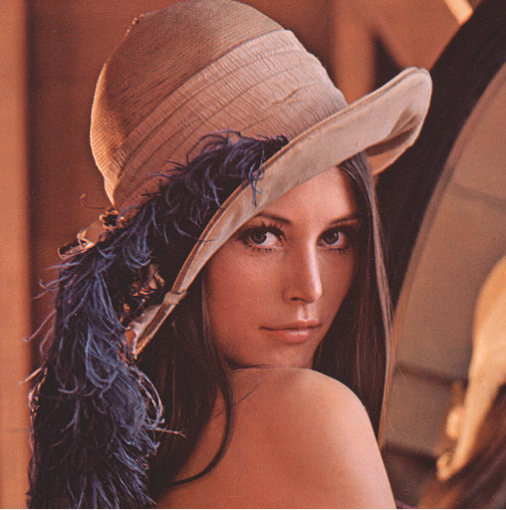
\includegraphics[width=3cm, height=3cm]{images/lena.png}\\\\

  \hline

 act1 &  gray  & image & oact1& 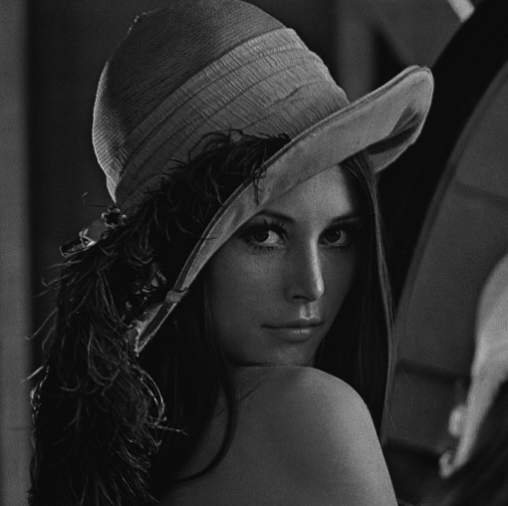
\includegraphics[width=3cm, height=3cm]{images/1.png}\\

   \hline

  act2 & Gaussian & image1 & image2 & 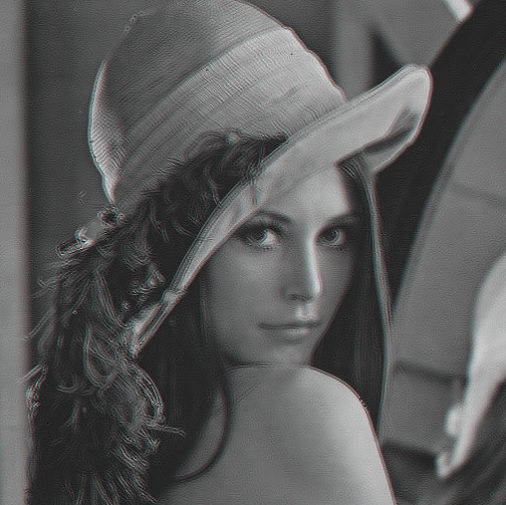
\includegraphics[width=3cm, height=3cm]{images/2.png}\\

  \hline

    act3 & Sobel & 2.3 & image3 & 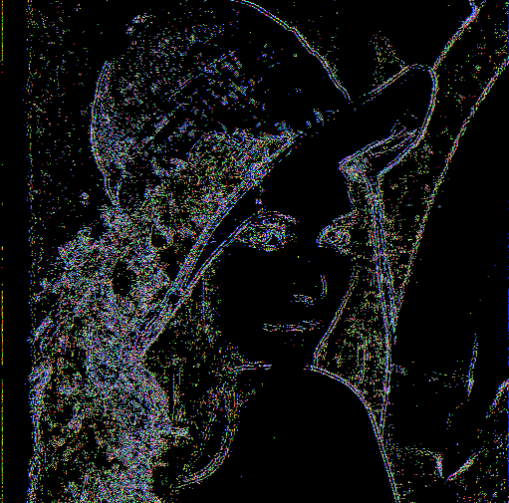
\includegraphics[width=3cm, height=3cm]{images/3.png}\\

  \hline

    act4 & Non-max & image3  & image4 &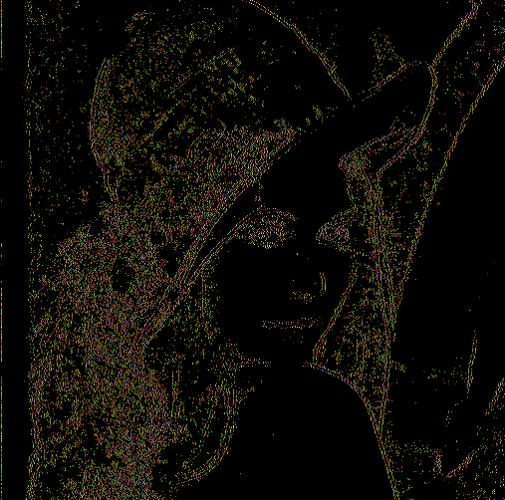
\includegraphics[width=3cm, height=3cm]{images/4.png} \\

  \hline

    act5 & hysteris & mage4 & image5 & 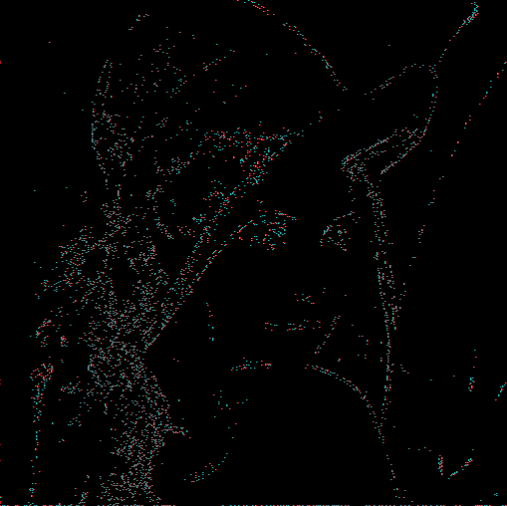
\includegraphics[width=3cm, height=3cm]{images/5.png}\\

  \hline

\end{tabular}
\caption{Le flux de travail de canny}
\end{table}

 %\section{Annexe}
%Ce troisième chapitre s'intéresse à présenter le domaine de workflow scientifique.

%\subsection{workflow scientifique}
%Le concept de workflow structure le processus de simulation scientifique comme un graph d'activities, dans lequel les noeuds correspondent aux activitiés de calcul numérique et les arêtes représentent le flux de données entre eux. les activités du workflow sont associées aux programmes qui préparent et analysent les données\cite{oga11}, on appel ces programmes des activations. 

% \vspace{0.25cm}
%\subsection{Les systèmes de gestion de workflow scientifique}
%Ce sont des systèmes de gestion de flux de travail (scientifique workflow management system) qui supportent la définition, l'exécution et la simulation des workflow scientifique\cite{oga11}.

\appendix
\chapter{Logiciels}
Durant ce stage on s'appuie principalement sur deux logiciels :
\begin{description}\label{chiron}
\item[Chiron]  \url{http://chironengine.sourceforge.net/}.

Chiron est un système de gestion de flux de travail de calculs numériques (\textit{scientifique workflow management system}),  il exécute ces simulations comme une chaîne d'activités (programmes) et un flux de données (dataflow) sur ces activités. Ce système fournit la gestion des simulations scientifiques, leur exécution parallèle tout en enregistrant la provenance des données. Chiron implémente l'approche algébrique dans un style MapReduce. L'utilisation de MapReduce comme approche de programmation permet aux scientifiques de programmer d'une façon plus simple la procédure du calcul en cachant le parallélisme, qui peut être complexe à gérer \cite{oga13}.


\item[SPOC] \url{http://www.algo-prog.info/spoc/}.

SPOC (Stream Processing with OCaml)  consiste en une extension à OCaml associée à une bibliothèque d'exécution. L'extension permet la déclaration de noyaux GPGPU externes utilisables depuis un programme OCaml, tandis que la bibliothèque permet de manipuler ces noyaux ainsi que l'automatisation des transferts de données nécessaires à leur exécution. SPOC offre, de plus, une abstraction supplémentaire en unifiant les deux environnements de développement GPGPU (Cuda et OpenCL) en une même bibliothèque \cite{bou14}, \cite{bour14}.


\end{description}
\vspace{0.5cm}

%\begin{description} c'est quoi la logiciel
%\item[GPU] NVIDIA Corporation GF108GLM [Quadro 1000M].
%\end{description}
\vspace{\parskip}
%\end{flushleft}



\bibliographystyle{plain}
\bibliography{biblio}

%\newpage
\thispagestyle{empty}
\tableofcontents
%\thispagestyle{empty}

%\selectlanguage{french}
%%\include{Chapters/resum}
%\newpage




\end{document}
